% Here we have your executive summary.
This thesis describes a new method for measuring strain dependent surface stress in soft solids, as well as the corresponding measurements for variety of silicone. Over the past several years, recent attempts to measure surface stress in gels have returned a cornucopia of conflicting results, differing significantly in similar materials. Professor Katharine Jensen suggested that this discrepancy is an artifact of the strain state of the gels, and recently made the first ever measurement of strain-dependent surface stress, $\Upsilon(\epsilon)$, in solids \cite{xu2017direct}. In this 2017 Nature Communications paper, Professor Katharine Jensen and her colleagues at ETH Zürich reported that the surface stress changed dramatically under applied strain. At 18\% strain, the surface stress more than doubled. 
\begin{figure}[h!]
	\centering
	\textbf{Should I give it a title?}\par\medskip
	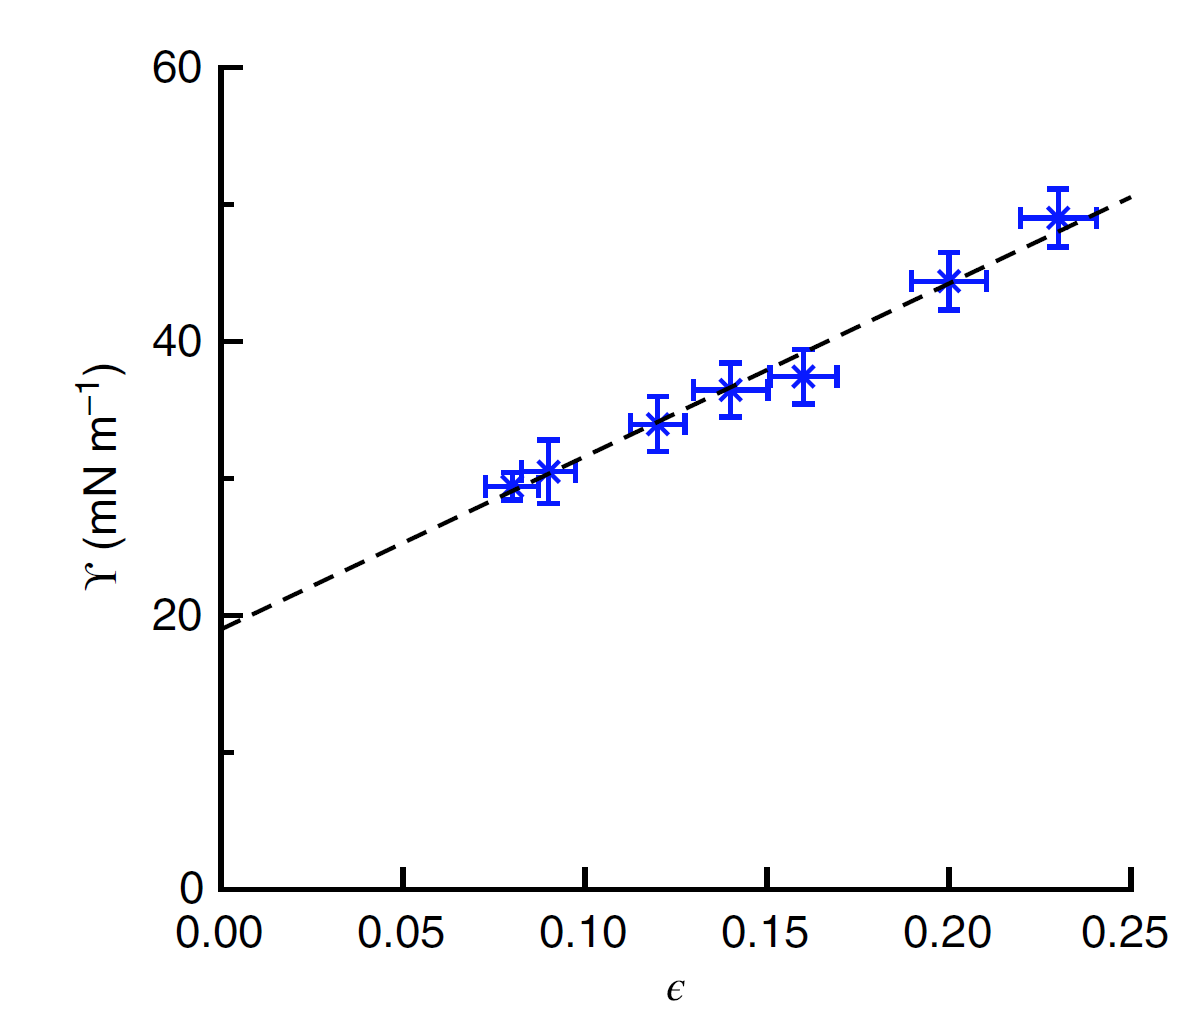
\includegraphics[width=0.7\linewidth]{Chapters/Figures/2017natcomfig}
	\caption[Surface Stress vs. Strain in Silicone]{First direct measurement of strain dependent surface stress in solids \cite{xu2017direct}}
	\label{fig:2017natcomfig}
\end{figure}

Over the past year, we have helped develop a new and superior method for measuring $\Upsilon(\epsilon)$ in soft solids. Unlike the previous techniques, our adhesion-based method can be applied to virtually any soft solid capable of being stretched. We have also build our own equibiaxial stretching apparatus, improving upon the earlier published design \cite{xu2017direct} to produce nearly twice the strain in identical materials. The goal of this thesis has been to develop and hone an adhesion based technique for measuring strain dependent surface stress in soft solids. Using this technique, we then can recreate the controversial 2017 measurements to add validity both to our technique and to the picture that surface stress varies significantly under strain in gels.

\emph{Next I will talk about the [hopefully] awesome results I get with Dow Corning and include a figure there. I leave the rest of this section for the }


%From Charlie:
%Your executive summary will give a detailed summary of your thesis, hitting the high points and perhaps including a figure or two.  This should have all of the important take-home messages; though details will of course be left for the thesis itself, here you should give enough detail for a reader to have a good idea of the content of the full document.  Importantly, this summary should be able to stand alone, separate from the rest of the document, so although you will be emphasizing the key results of your work, you will probably also want to include a sentence or two of introduction and context for the work you have done.


